\subsection{Forma del fascio}

Abbiamo fatto delle misure di conteggio a vari angoli con e senza collimatori per studiare la forma del fascio.

\subsubsection{Assenza di collimatori}

La misura in assenza di collimatori ci permette di indagare la forma del fascio di particelle $\alpha$ in uscita dalla sorgente di \am{}.
\marginpar{disegno provvisorio}
Bisogna notare che l'angolo segnato sulla scala graduata non coincide con quello tra la sorgente ed il rivelatore perché il fotodiodo non è al centro della camera a vuoto, inoltre all'aumentare (in modulo) dell'angolo la distanza tra sorgente e rivelatore diminuisce. 
Lo schema di \autoref{fma} illustra la situazione.

\begin{figure}[h]
\centering
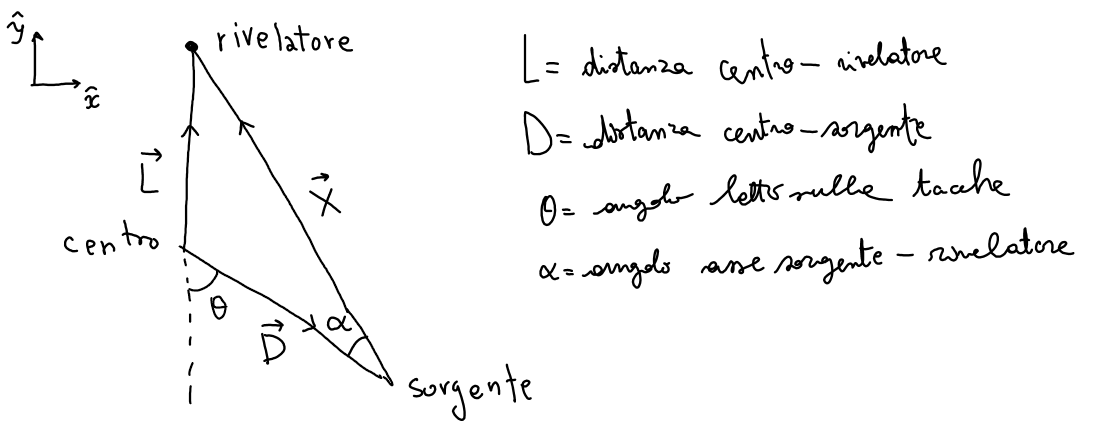
\includegraphics[width=30 em]{immagini/fma_provv}
\caption{Schema raffigurante gli angoli tra rivelatore, centro della camera a vuoto e sorgente.}
\label{fma}
\end{figure}

Applicate le dovute correzioni e usando le variabili di \autoref{fma} troviamo che l'angolo tra rivelatore e sorgente è
\begin{equation}
\cos{\alpha}= -\frac{\vec{X} \cdot \vec{D} }{ |\vec{X}| |\vec{D}| } = \frac{ L \cos{\theta} + D }{ \sqrt{ L^2+2LD\cos{\theta}+D^2  } }.
\end{equation}

Teniamo conto della variazione della distanza al variare dell'angolo moltiplicando ogni rate per $|\vec{X}|^2$.
Tale fattore è giustificato dal fatto che supponiamo isotropa l'emissione di particelle $\alpha$ da parte della sorgente.
Se $C$ è una costante, abbiamo che $$ \frac{dN}{d^3r}=C \implies \frac{dN}{dr}=C 4\pi r^2. $$

\marginpar{A dire il vero non lo so perché. Mi sembra che bisogna dividere per X$^2$ (analogia col campo elettrico). Invece moltiplichiamo. Il grafico ha senso ma non mi torna perché dovrei avere meno eventi all'allontanarmi dal rivelatore ad angolo fissato.}

Il risultato di questa misura è presente in \autoref{fig:form}, invece la \autoref{tab:form} contiene i dati di tale grafico.
Si evince che il fascio ha un'estensione angolare di quasi \SI{50}{\degree}.

\marginpar{inserire tante belle cose}

Useremo queste informazioni (se sarà necessario) nell'analizzare i dati sulla sezione d'urto.

\subsubsection{Collimatore da 5\! mm}

\subsubsection{Collimatore da 1\! mm}

\subsubsection{Collimatore a croce}